\begin{figure}[t]
  \centering  
  \includegraphics[width=0.45\textwidth]{\main/Flavour/figs/mixing_Bs}~~~~
  \raisebox{1.5mm}{\includegraphics[width=0.45\textwidth]{\main/Flavour/figs/mixing_Bs_NP}}
  \caption{Examples of diagrams contributing to $B_s-\bar B_s$ mixing in the SM (left) and example of SUSY new physics contributions, with a gluino-squark exchange shown as an example (right), adapted from \cite{Zupan:2019uoi}.}
  \label{fig:Bsmixing}
\end{figure}

The flavour physics results obtained at the LHC in the past decade have far exceeded expectations. 
A combination of measurements by LHCb and CMS resulted in the observation of the long sought-after $B_s\rightarrow \mu^+\mu^-$ decay mode in 2014~\cite{CMS:2014xfa}.
Remarkable progress has been made in CP violation studies in the beauty sector including  measurements of the CKM angle $\gamma$ by LHCb~\cite{Aaij:2018uns}, 
$B_s$ mixing phase $\phi_s$ by ATLAS and LHCb~\cite{ATLAS:2019akj,Govorkova:2019jlz}, and the discovery of CP violation in the $B_s$ system by LHCb~\cite{Aaij:2013iua}.
In charm physics, a landmark result was obtained by LHCb in 2019 with the observation of CP 
violation~\cite{Aaij:2019kcg}, opening a new field of study. Spectroscopic studies also yielded important results, with several new hadronic states found by the LHCb, including the observation of pentaquark states ~\cite{Aaij:2015tga,Aaij:2019vzc} in 2014 and 2019.

An important goal of the program is to search for potential new physics effects that could enter through virtual corrections, see Fig. \ref{fig:Bsmixing} for a $B_s-\bar B_s$ mixing example. It is important to stress that there are a number of measurable quantities that are {\it theoretically clean}, and where the knowledge will still be statistically limited after Belle II and LHCb Upgrade I. A list of such observables, which will actively drive the field, includes the CP-violating phase $\gamma$, the lepton-universality ratios $R_{K^{(*)}}$, $R_{D^{(*)}}$,  etc., the mixing phase in the $B_s$ and $D$ systems, as well as the ratio of branching ratios ${\rm{BR}} (B_d \rightarrow \mu^+ \mu^-)$/${\rm{BR}} (B_s \rightarrow \mu^+ \mu^-)$. 
A notable target of the physics programme at the \HLLHC is to probe at the $10\%$ level the ratio ${\rm{BR}}(B_d \to \mu^+\mu^-)/ {\rm{BR}}(B_s \to \mu^+\mu^-)$, which, in case that new physics deviations are found, is a powerful observable to test the MFV hypothesis. The combined sensitivity of ATLAS, CMS and LHCb are shown in  Fig.~\ref{fig:Bmumu} (upper panel).  

Intriguingly, some measurements, in both charged-current and neutral-current 
semileptonic \textbf{$B$ decays}, hint at a violation of one of the 
key predictions of the SM: the universality of interactions for leptons of different generations (\textbf{LFUV}). 
The statistical significance of the anomalies is not sufficiently high to 
claim a discovery, but the situation is very interesting. Regardless of whether or not their statistical significance increases with improved measurements, the anomalies do demonstrate the genuine discovery potential of the flavour programme at the LHC.
More precise measurements of some of these observables, in particular the  
 LFUV ratios
$R_{K^{(*)}} = \Gamma(B\to K^{(*)} \mu^+\mu^-) / \Gamma(B\to K^{(*)} e^+e^-)$ and 
$R_{D^{(*)}} = \Gamma(B\to D^{(*)} \tau\bar\nu) / \Gamma(B\to D^{(*)} \ell\bar\nu)$, where $\ell=e,\, \mu$,
could establish the presence of new physics, even 
with modest improvements in statistics.  
The current experimental situation for 
$R_{K}$~\cite{PhysRevLett.103.171801, PhysRevD.86.032012,PhysRevLett.113.151601,Aaij:2019wad,Abdesselam:2019wac} is shown in Fig.~\ref{fig:RKRD} (upper panel), and for $R_{D^{(*)}}$~\cite{Abdesselam:2019dgh,PhysRevD.97.072013,PhysRevLett.118.211801, PhysRevLett.115.111803,PhysRevD.94.072007,PhysRevD.92.072014,PhysRevD.88.072012,PhysRevLett.109.101802,Aaij:2017uff} in Fig.~\ref{fig:RKRD} (lower panel). While the discrepancies are still not statistically significant, it may be useful to address which type of new physics could explain them if they do become significant.  
To explain the $R_{D^{(*)}}$ discrepancy, new physics needs to enter at tree-level and be lighter than a few TeV, while for $R_{K^{(*)}}$ the tree-level new physics can be as heavy as several tens of TeVs, such as a $Z'$ with ${\mathcal O}(1)$ couplings. A combined explanation of both sets of anomalies is possible using leptoquarks. 
Interestingly, some tensions with the SM predictions are also seen in the $B \to K^{*} \mu^+\mu^-$ angular distributions \cite{Aaij:2015oid,Wehle:2016yoi,Sirunyan:2017dhj,Aaboud:2018krd}, possibly forming a coherent pattern with the LFUV measurements. However, compared to LFUV ratios the SM predictions in this case do have larger uncertainties due to the presence of charm-loops, making reliable theoretical description essential for future progress \cite{Jager:2012uw,Ciuchini:2017mik,Matias:2012xw,DescotesGenon:2012zf,Bobeth:2017vxj}.

In the {\bf short-term}, significant progress is expected in the precision of the measurements for core flavour physics observables, whose knowledge is still largely statistically limited. There is a concerted effort devoted to extensive studies of the $b\rightarrow s \ell^+\ell^-$, $b\rightarrow d \ell^+\ell^-$ and $b \rightarrow c \ell^- \bar\nu_\ell$ transitions, including analysis of $B$-hadron decay angular distributions. 
%
The two dedicated $B$-physics experiments, Belle~II, the $e^+e^-$ superflavour factory 
operating mostly at the $\Upsilon(4S)$ resonance, and the LHCb at the LHC, including its Upgrade~I,
are aiming at a rich programme of measurements to be performed, {\bf with a high level of complementarity}.  LHCb benefits from higher statistics in charged-track decay modes and the access to all $b$ hadrons, while Belle~II has a unique access to fully neutral final states and rare leptonic decays with final state neutrinos. 
The ATLAS and CMS experiments 
will continue to contribute to flavour physics, notably in $B$ decays to final states containing muons.
\begin{figure}[t]
  \centering  
  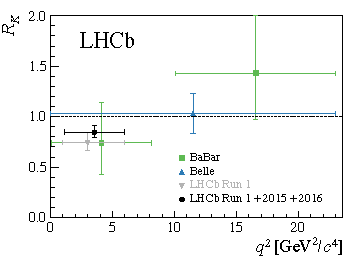
\includegraphics[width=0.7\textwidth]{\main/Flavour/figs/RKLHCb.pdf}\hbox{\hspace{-0.2cm}}\\
  \includegraphics[width=0.715\textwidth]{\main/Flavour/figs/rdrds_spring2019.png}\hbox{\hspace{-0.2cm}} 
  \caption{Upper panel: experimental results for 
  $R_K$ as function of the di-lepton invariant mass squared, $q^2$. Lower panel: status of $R_{D^{(*)}}$
  measurements; the SM predictions are  
   in tension with the experimental world average at 
  the 3.08\,$\sigma$ level \cite{HFLAVSPRING19}.}
  \label{fig:RKRD}
\end{figure}

\begin{figure}[t]
\centering
\includegraphics[width=0.45\textwidth]{\main/Flavour/figs/B2MuMu_HL-LHC.pdf}\\
\includegraphics[width=0.4\textwidth]{\main/Flavour/figs/YR_C9_C10.pdf}
\caption{ 
Upper panel: BR$(B_s^0 \to \mu^+\mu^-)$ vs. BR$(B_d^0 \to \mu^+\mu^-)$ in the SM (black cross), and in a particular supersymmetric unified model (green points are consistent with other constraints). The coloured contours show the expected $1\sigma$ \HLLHC sensitivity of ATLAS, CMS, and LHCb Upgrade~II. Lower panel: combined sensitivity of LHCb, ATLAS and CMS after the \HLLHC phase to potential new physics in $b\to s\mu\mu$ processes, motivated by recent anomalies. New physics benchmarks with leptonic vector current (new physics only in $C_9$) or pure left-handed current ($C_9=-C_{10}$), as well as the SM predictions are shown. The observables included are the branching ratio  of the $B_s\to\mu^+\mu^-$ decay and the angular observables of the decay $B^0 \to K^{\ast 0} \mu^+\mu^-$ in the low-$q^2$ region.
See  Ref.~\cite{Cerri:2018ypt} for details.}
\label{fig:Bmumu} 
\end{figure} 

In the {\bf mid-term}
the LHCb Upgrade~II, combined with the enhanced $B$-physics capabilities of ATLAS and CMS Phase~II upgrades, will enable a wide range of flavour observables to be determined at \HLLHC with unprecedented precision, complementing and extending the reach of Belle II, and of the high-p$_T$ physics programme.
Substantially improved tracking systems and the addition of timing layers in ATLAS and  CMS Phase-II detectors may significantly improve their capabilities for charged-hadron  particle identification.
The LHCb Upgrade~II will allow the experiment to run at instantaneous luminosities up to $2 \times 10^{34}{\rm cm}^{-2} {\rm s}^{-1}$ with a target integrated luminosity of 300 fb$^{-1}$, and thus exploit the full \HLLHC potential in flavour physics \cite{Bediaga:2018lhg, Cerri:2018ypt}.
Generically, and for fixed couplings, the new physics mass scale probed  will roughly double compared to the pre-\HLLHC era, see Fig.~\ref{fig:NPscales} (light vs.\ dark green for mid-term prospects with LHCb Upgrade~II).

Very recently, the suggestion that a factor of five increase in luminosity could be achieved at SuperKEKB was raised, aiming for an integrated luminosity of $250~{\rm ab}^{-1}$.
The clear complementarity of flavour physics at $e^+ e^-$ and "$pp$" colliders makes this possibility appealing. 
The major issues related to such Belle~III project  
are the feasibility from accelerator perspective and the detector challenges when running at 4 $\times 10^{36}$
cm$^{-2}$ s$^{-1}$.

The \HLLHC, combining ATLAS, CMS and LHCb Upgrade~II, has the potential to distinguish between some well-motivated  
new physics scenarios. 
The increasing precision of observables from measurements of statistically limited FCNC processes will provide significant improvements in terms of the reach to the energy scale of new-physics. 
As an example, the  plot in Fig.~\ref{fig:Bmumu} (lower panel) shows the potential sensitivity to the Wilson coefficients $C_9$ (vector current) and $C_9=-C_{10}$ (pure left-handed current), for definitions see, e.g., \cite{Aebischer:2019mlg}.
These fit results take as inputs the measurements of the branching ratio of the  $B_s\to\mu^+\mu^-$ decay and the angular observables from the decay $B^0 \to K^{\ast 0} \mu^+\mu^-$ in the low-$q^2$ region. The reach for generic new physics at tree-level is found to exceed 100~TeV, and in terms of the constraints on new-physics contributions to the $C_9$ and $C_{10}$ Wilson coefficients the study shows an approximate gain of about a factor of two compared to the constraints prior to \HLLHC. 

In addition, a wide range of lepton-universality tests in $b \to c \ell \nu$ decays can be performed, exploiting the full range of
$B$ hadrons, to probe  models of new physics.
The copious yields of semileptonic decays allow the high-precision search for CP violation in $B^0$ and $B_s$ mixing. 
In the {\bf mid-term}, the LHCb Upgrade~II dataset will allow the semileptonic asymmetries for both mesons to be measured at the level of a few $10^{-4}$, giving unprecedented new-physics sensitivity.
Precise measurements of \textbf{${\phi_s}$} and 
\textbf{${\sin 2 \beta}$} will be performed, with strategies to monitor and control possible  pollution from penguin contributions.
Advances in lattice-QCD calculations will also motivate better measurements of other critical observables, e.g., $|V_{ub}|/|V_{cb}|$, for details see Section  \ref{sec:CKM_prospects}. 

In the {\bf long-term},
at future colliders, the heavy-flavour physics is expected to be, as it is now, an integral part of the physics programme.
The new $e^+e^-$  circular colliders 
are foreseen to collect 
 $\sim 10^{ 11}$ and 
 $ \sim  10^{12}$ 
 $Z \to b \bar b$ events at 
\CEPC \cite{CEPC_INPUT} and \FCCee  \cite{Blondel:2019yqr} respectively, which  will result in all species of heavy-flavoured hadrons.
 The boosted topologies of the decay particles at the $Z$ energy, in conjunction with the clean $e^+e^-$ environment, will be beneficial for a number of measurements. 
In this respect, the $B_{s,d} \to \tau^+\tau^-$ and  $ B \to K^{(*)} \tau^+ \tau^-$ decays are  natural candidates to study. For example about 1000  events with a reconstructed  $\bar {B}^0 \to K^{*0} \tau^+\tau^-$ are expected in the $5 \times 10^{12}$ $Z$ decays at \FCCee, which would 
allow for the first investigation of  the tau lepton polarization in this mode 
\cite{Kamenik:2017ghi}. 
Recently, there has been renewed interest for the GigaZ programme at a linear collider, i.e., for runs that would collect $\sim 10^9 Z$'s from collisions with polarized electrons~\cite{Irles:2019xny}.
In general, TeraZ samples  of $\ge 10^{12} Z$'s are needed to further improve flavour-physics precision measurements and searches for rare decays after the LHCb Upgrade~II and   Belle~II (and possibly Belle~III).  
In particular, three different tests of lepton universality can be performed at a $Z$-factory. Charged current universality tests are best carried out with the $1.7 \times 10^{11}  \tau^+ \tau^-$ pairs (precision level $10^{-5}$ with TeraZ samples).
Further tests can be also performed using rare decays of heavy-flavour hadrons from the $\sim 10^{12}$ $Z\to b\bar b$  and $Z\to c \bar c$ decays.
In this case there is no benefit from the longitudinal polarization so that the polarized GigaZ sample, with three orders of magnitude fewer events, is significantly more limited. 
Neutral current universality can be tested first from the comparison of the partial widths of the $Z$ into each of the three lepton pairs; a precision better than $10^{-5}$ is expected at the TeraZ. Here again, the GigaZ will  suffer from 3000 times less statistics. 
 The ratio of vector-to-axial-vector couplings can be accessed through measurements of initial- and final-state polarization asymmetries, as well as forward-backward asymmetries. For such asymmetry measurements  the initial-state beam polarization brings substantial improvements in the reach. However, these measurements can be well performed also without longitudinal beam polarization 
 \cite{Blondel:2019yqr}.

In the \FCChh configuration, a dedicated experiment  \`{a} la LHCb could be conceived, for instance at the booster stage of the accelerator complex. Since a number of observables are expected to have negligible theoretical uncertainties even when compared with the experimental ones  after LHCb Upgrade~II, there could be a strong physics case for such an experiment.



The discussion so far focused on the physics with $b$ quarks. A related, yet different probe of new physics is offered by the {\bf charm quark decays}. In the SM, the FCNC processes involving charm hadrons are suppressed compared to those involving strange or beauty hadrons, in both the mixing and decay amplitudes. The reason is, on the one hand, that the charm quark, unlike the $b$ and $s$ quarks, can decay inside its own family. The characteristic time for the FCNC transitions is therefore much longer than the decay time, giving both $\Delta M/\Gamma\ll~1$ and $\Delta \Gamma/\Gamma\ll~1$. This fact is sustained, on the other hand, by the small breaking of the GIM mechanism controlled by the $b$ quark mass. 
The charm FCNCs can then be used as sensitive probes of new physics in the up-quark
sector, to the extent that theoretical uncertainties can be brought
under control, e.g., by constructing null tests, or circumvented by using the experimental data.

In the SM, the size of CP violation in charm decays is predicted  to be $\mathcal{O} (10^{-3} -10^{-4}$), and may be altered by  virtual new physics particles. 
The first observation of CP violation in the decay of charmed hadrons \cite{Aaij:2019kcg}
opens new opportunities across two-body, multi-body, direct and indirect CPV. The projected precisions of some analyses performed by LHCb are shown in   Fig.~\ref{fig:charm_indirect_channels} (upper panel) and are compared with the {\bf short-} and {\bf mid-term} precisions expected at Belle~II and \HLLHC. 
The available experimental measurements are also combined to establish the sensitivity to the CP-violating parameters $q/p$ and $\phi$. 
The lower plot in Fig.~\ref{fig:charm_indirect_channels}  shows the projected sensitivity with the HFLAV world average as of 2017.
At an integrated luminosity of $300\invfb$ the sensitivity to $|q/p|$ is expected to be $0.001$ and that to $\phi$ to be $0.1^\circ$.
The LHCb \upgradetwo will have the power to reach the SM estimates for $\phi$, and characterise possible new-physics contributions, if these are not too suppressed.
The charm sector investigation will be  exploited at BESIII, LHC, Belle~II (Belle~III) and \HLLHC. The programme could be complemented by some specific initiatives: TauFV at the Beam Dump at CERN \cite{TauFV_input} and $e^+e^-$ SCT factories. 
BESIII, and possibly future charm-tau factories, will exploit the $e^+e^- \to D^0 \bar {D^0}$ process to perform quantum-correlation measurements.
\begin{figure}
  \centering
  \includegraphics[width=0.85\textwidth]{\main/Flavour/figs/CharmIndirectCPVSummary.pdf}\vspace*{3mm}\\
 \includegraphics[width=0.65\textwidth]{\main/Flavour/figs/charm_indirect_CPV.pdf} 
  %
  \caption{Upper panel: Predicted constraints on the indirect CP violation
    asymmetry in
    charm from the decay channels indicated in the labels at the
    bottom of the columns. Predictions are shown in LS2
    (2020) from LHCb, LS3 (2025) from LHCb, at the end of Belle~II (2025), and at the end
    of the \HLLHC LHCb Upgrade~II\ program.
    Lower panel: Estimated constraints for LHCb \upgradetwo\ on $\phi$, $|q/p|$ from the combination of the analyses (red) compared to the current world-average precision (light blue).} 
\label{fig:charm_indirect_channels}
\end{figure}

